\documentclass{mcmthesis}
\mcmsetup{CTeX = false,   % 使用 CTeX 套装时,设置为 true
        tcn = 2013647, problem = D,
        sheet = true, titleinsheet = false, keywordsinsheet = true,
        titlepage = false, abstract = true}
    
\usepackage{palatino}
\usepackage{lipsum}
\usepackage{fancyhdr}
\usepackage{extramarks}
\usepackage{amsmath}
\usepackage{amsthm}
\usepackage{amsfonts}
\usepackage{tikz}
\usepackage[plain]{algorithm}
\usepackage{algpseudocode}
\usepackage{arydshln}
\usepackage{mathtools}
\usepackage{cases}
\usepackage{listings}
%\usepackage[numbered]{mcode}
\usepackage{booktabs}
\usepackage{graphicx}
\usepackage{subfigure}

\title{The \LaTeX{} Template for MCM Version \MCMversion}
\date{\today}
\begin{document}
\begin{abstract}
\lipsum[1]
\begin{keywords}
keyword1; keyword2
\end{keywords}
\end{abstract}
\maketitle
%% Generate the Table of Contents, if it's needed.
%% \tableofcontents
%% \newpage
%%
%% Generate the Memorandum, if it's needed.
%% \memoto{\LaTeX{}studio}
%% \memofrom{Liam Huang}
%% \memosubject{Happy \TeX{}ing!}
%% \memodate{\today}
%% \logo{\LARGE I'm pretending to be a LOGO!}
%% \begin{memo}[Memorandum]
%%   \lipsum[1-3]
%% \end{memo}
%%
\tableofcontents
\section{Introduction}
	
	\subsection{Background}
	
	\subsection{Problem Description}
	
	\subsection{General Assumptions}
		
	\subsection{Notation}


\section{Analysis of the Problem}
	\subsection{Correlation Analysis and Heat Map}
		According to the data given, we computed the correlation among the passing position, event type, event sub type and the outcome. Here we use the $\phi$ coefficient of chi-squares test, where $\phi=\sqrt{\frac{\mathcal{X}^2}{n}}$. The advantage of using $\phi$ coefficient is it can test the association between several variables and is always bigger than zero. The following is the result. 
		\begin{figure}[h!]
			\centering
			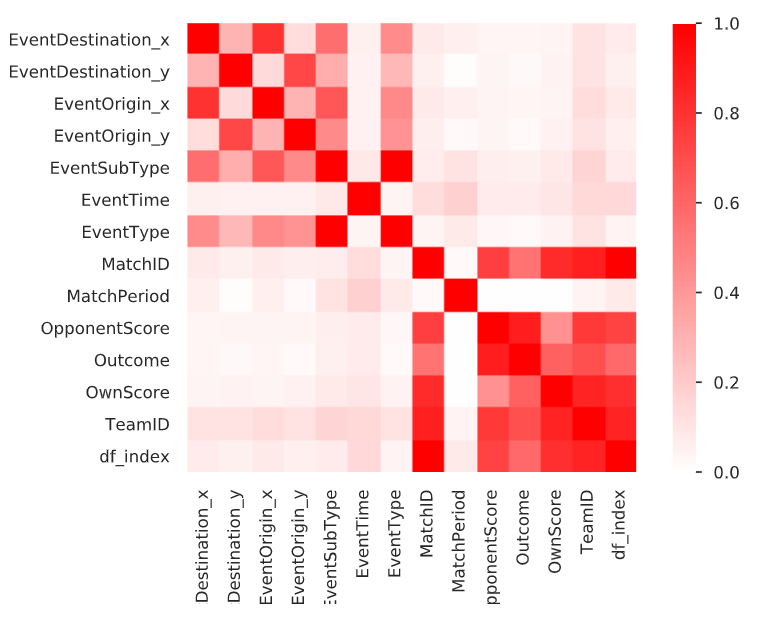
\includegraphics[scale=0.6]{images/cor_1.PNG}
			\caption{$\phi_k$ coefficient between different variables. }
		\end{figure} \\
		We can see that the area of passing position and outcome has very weak association. 
		
		
	\subsection{Network Analysis}
	
\section{Network Display}


\section{Build Network Science Model}

\section{Model Validation}

\section{Validating the Model}


\section{Conclusions}


\section{A Summary}


\section{Evaluate of the Mode}

\section{Strengths and weaknesses}


\subsection{Strengths}


\begin{thebibliography}{99}
\bibitem{1} D.~E. KNUTH   The \TeX{}book  the American
Mathematical Society and Addison-Wesley
Publishing Company , 1984-1986.
\bibitem{2}Lamport, Leslie,  \LaTeX{}: `` A Document Preparation System '',
Addison-Wesley Publishing Company, 1986.
\bibitem{3}\url{http://www.latexstudio.net/}
\bibitem{4}\url{http://www.chinatex.org/}
\end{thebibliography}

\begin{appendices}

\section{First appendix}

\lipsum[13]

Here are simulation programmes we used in our model as follow.\\

\textbf{\textcolor[rgb]{0.98,0.00,0.00}{Input matlab source:}}
\lstinputlisting[language=Matlab]{./code/mcmthesis-matlab1.m}

\section{Second appendix}

some more text \textcolor[rgb]{0.98,0.00,0.00}{\textbf{Input C++ source:}}
\lstinputlisting[language=C++]{./code/mcmthesis-sudoku.cpp}

\end{appendices}
\end{document}

%% 
%% This work consists of these files mcmthesis.dtx,
%%                                   figures/ and
%%                                   code/,
%% and the derived files             mcmthesis.cls,
%%                                   mcmthesis-demo.tex,
%%                                   README,
%%                                   LICENSE,
%%                                   mcmthesis.pdf and
%%                                   mcmthesis-demo.pdf.
%%
%% End of file `mcmthesis-demo.tex'.
